\chapter{Procesbeheer}\label{procesbeheer}

Een computersysteem voert programma's uit. De gebruiker wil
programma's kunnen opstarten, tijdelijk onderbreken en afsluiten. Meerdere
programma's tegelijk uitvoeren en eventueel prioriteiten toekennen moet
ook mogelijk zijn.

\section{Processen}

Een \emph{proces}\index{proces} is niet hetzelfde als een
programma. Een proces is een programma in uitvoering. Een programma is
niet meer dan uitvoerbare code.

Wanneer zo'n programma uitgevoerd wordt moet de code in het
werkgeheugen geladen worden, maar er moet ook plaats zijn voor b.v. de
waarden van de variabelen tijdens de uitvoering.

Wanneer een programma uitgevoerd wordt omvat het proces
verschillende componenten. Er is een gereserveerd deel van het geheugen,
met daarin de uit te voeren code, maar ook de waarden van variabelen. De
processortoestand omvat de inhoud van de bevelenteller en verschillende
registers. Het besturingssysteem houdt ook gegevens bij om de uitvoering
te kunnen organiseren, zoals b.v. de bestandsbeschrijvingen van
bestanden die door het proces geopend zijn of de eigenaar en de
toegangsrechten van het proces.

Eenzelfde programma kan tegelijkertijd door verschillende
processen uitgevoerd worden, zoals de schermafdruk illustreert. Dan moet
voor iedere uitvoering een apart deel van het geheugen beschikbaar zijn
om de toestand van het proces bij te houden.

\subsection{Multiprogrammatie}

Een processor kan maar \'e\'en programma tegelijkertijd uitvoeren.
Als we toch meerdere processen willen uitvoeren is de meest voor de
hand liggende oplossing meerdere processoren gebruiken. Maar als het
aantal gelijktijdige processen groeit, stijgt ook het aantal
processoren dat we nodig hebben. Dit is natuurlijk een te dure
oplossing voor een eenvoudig computersysteem. Bovendien zullen een
aantal van de processoren stilstaan als niet het maximum aantal
gelijktijdige processen beschikbaar is voor uitvoering.

Als we op een uniprocessor-systeem op hetzelfde ogenblik
meerdere processen willen uitvoeren, moeten we het
\emph{multiprogrammatie}\index{multiprogrammatie} principe toepassen. De
rekentijd op \'e\'en processor wordt dan verdeeld over meerdere processen.
De processen kunnen om beurt voor een bepaalde tijd gebruik maken van
de processor.

Het kan gaan om verschillende processen van dezelfde gebruiker.
Als we verschillende gebruikers tegelijkertijd op \'e\'en processor laten
werken door hun processen via multiprogrammatie uit te voeren spreken
we van \emph{timesharing}\index{time sharing}. Het lijkt alsof
verschillende processen tegelijkertijd verwerkt worden, maar in
werkelijkheid wisselt de processor van het ene proces naar het andere.
Het is het besturingssysteem dat de uitvoering van meerdere processen
gaat verweven om het processorgebruik te maximaliseren en tegelijk te
zorgen voor een aanvaardbare responstijd. Het onderdeel van het
besturingssysteem dat deze taak verzorgt heet de
\emph{scheduler}\index{scheduler}.

\begin{figure}
\centering
\begin{subfigure}{.5\textwidth}
  \centering
  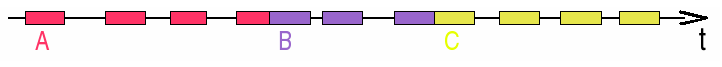
\includegraphics[width=100mm]{images/fig0501a.png}
  \caption{Zonder multiprogrammatie}
  \label{multprogr:a}
\end{subfigure}%
\begin{subfigure}{.5\textwidth}
  \centering
  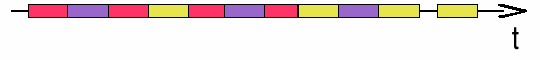
\includegraphics[width=75mm]{images/fig0501b.png}
  \caption{Met multiprogrammatie}
  \label{multprogr:b}
\end{subfigure}
\caption{Multiprogrammatie}
\label{multprogr}
\end{figure}

Als we geen gebruik maken van multiprogrammatie worden de
verschillende processen na mekaar uitgevoerd. Wanneer het proces in
uitvoering moet wachten op een externe gebeurtenis, zoals b.v. het
afwerken van een leesopdracht door een schijf of het resultaat van een
ander proces, staat de processor stil.

Door multiprogrammatie toe te passen kunnen we het
processorgebruik verbeteren. Als \'e\'en proces wacht op een gebeurtenis
kan de processor een ander proces uitvoeren.

In fig. \ref{multprogr} zien we duidelijk dat de processor bijna niet
meer werkloos is, alleen op het einde wanneer processen A en B
voltooid zijn is er geen ander proces beschikbaar om uit te voeren
terwijl C wacht. Merk op dat proces A eigenlijk nadeel ondervindt van
de multiprogrammatie, aangezien het nu later voltooid zal zijn.

Naast het optimaliseren van het processorgebruik zorgt
multiprogrammatie ook voor een lagere gemiddelde responstijd. De
\emph{responstijd} is de tijd tussen het geven van een
opdracht en het moment dat de ontvangst van het antwoord begint. Dit
is van belang bij interactief werken met een systeem. Bij timesharing
is het dus van belang om de responstijd zo laag mogelijk voor alle
gebruikers die het systeem delen.

Zoals we multiprogrammatie nu voorstellen blijven we een proces
uitvoeren tot het proces op een gebeurtenis wacht. Een proces dat zeer
veel rekenwerk moet doen, en weinig invoer- of uitvoeropdrachten bevat
waarop gewacht moet worden kan de processor dan relatief lang bezet
houden. Dit is slecht voor de gemiddelde responstijd omdat alle andere
processen dan zolang moeten wachten. Daarom zal het besturingssysteem
een proces soms na een bepaalde tijd onderbreken om andere processen
uit te kunnen voeren. Dit onderbreken noemen we
\emph{preemption}\index{preemption}.

\subsection{Toestanden van een proces}

Tijdens zijn uitvoering doorloopt een proces een aantal
toestanden. De overgangen tussen deze verschillende toestanden worden
teweeggebracht door de werking van het uitgevoerde programma ofwel
door de scheduler.

In het eenvoudigste geval zijn er twee toestanden: actief en
niet-actief. Een proces is actief als het uitgevoerd wordt door de
processor.

\begin{figure}
\begin{center}
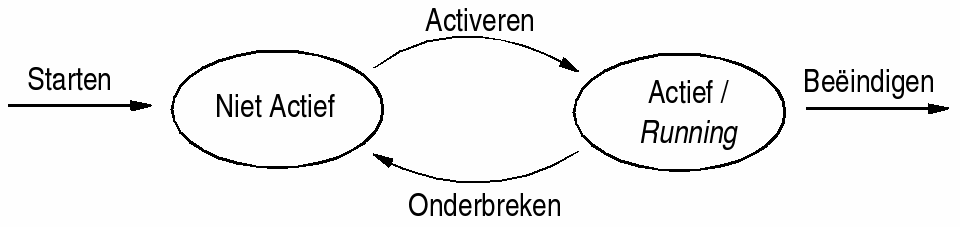
\includegraphics[width=100mm]{images/fig0502.png}
\caption{Twee toestanden van een proces}
\label{toestproc1}
\end{center}
\end{figure}

Wanneer een proces gestart wordt, zal het klaargemaakt worden
voor uitvoering en komt het in een niet-actieve toestand. De scheduler
zal dan een proces om uit te voeren kiezen uit alle niet-actieve
processen. Dit proces wordt dan actief. Wanneer het actieve proces
onderbroken wordt, en dus niet-actief wordt zal een ander proces
gekozen worden om uitgevoerd te worden.

Een proces wordt be\"eindigd als alle code is uitgevoerd. Omdat de
processor de code uitvoert kan een proces enkel aflopen vanuit de
actieve toestand. Wanneer het proces niet-actief is wacht het om
uitgevoerd te worden, en kan het dus nog niet be\"eindigd zijn.

Zoals reeds besproken zijn er 2 soorten onderbrekingen mogelijk
voor een proces in uitvoering. Enerzijds kan het proces door het
aanvragen van een invoer- of uitvoeropdracht moeten wachten. Dan wordt
het niet-actief. Anderzijds is er preemption, waarbij de scheduler het
actieve proces onderbreekt om een ander proces te kunnen starten. De
niet-actieve toestand moet dus opgesplitst worden in 2 aparte
toestanden: een geblokkeerd proces wacht op in- of uitvoer, en de
processen die gereed zijn kunnen door de scheduler gekozen worden om
uitgevoerd te worden.

\begin{figure}
\begin{center}
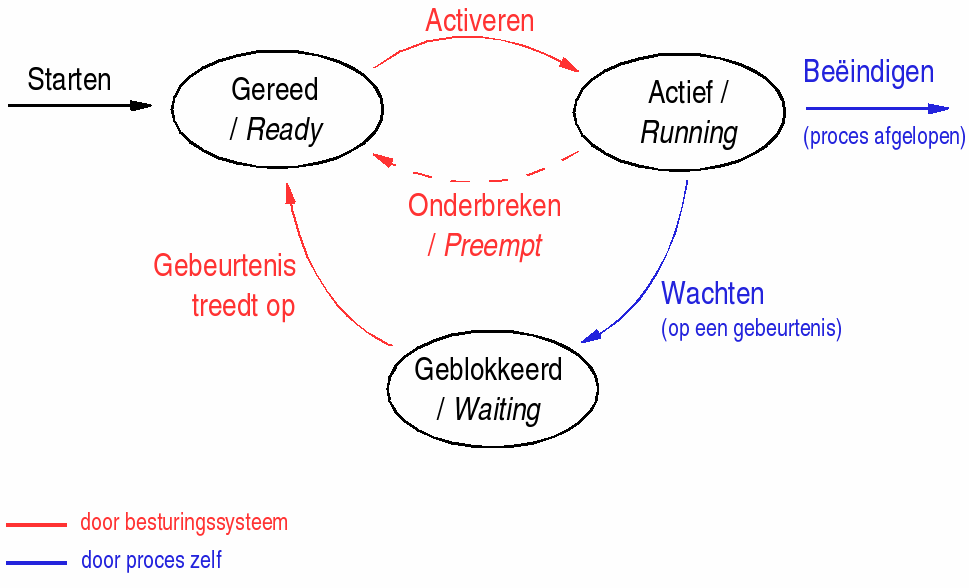
\includegraphics[width=100mm]{images/fig0503.png}
\caption{Drie toestanden van een proces}
\label{toestproc2}
\end{center}
\end{figure}


Processen die 'gereed' zijn, worden door het besturingssysteem
in een wachtrij bijgehouden. De scheduler kan uit deze wachtrij \'e\'en
proces activeren. Dit proces wordt dan actief en wordt door de
processor uitgevoerd. Er zijn drie manieren waarop een proces de
actieve toestand kan verlaten. Wanneer het proces afgelopen is zal het
natuurlijk niet langer actief zijn. Als het proces via een system call
een aanvraag doet waarvan het resultaat niet onmiddellijk beschikbaar
is zal het 'geblokkeerd' worden. Dit gebeurt dus op initiatief van het
proces zelf. Tenslotte kan ook het besturingssysteem een actief proces
onderbreken en terug aan de wachtrij toevoegen d.m.v. preemption. Dit
mechanisme is niet in alle systemen beschikbaar. Er zijn preemptive en
non-preemptive schedulers.

Processen die vaak in- en uitvoer nodig hebben, en dus vaak
'geblokkeerd' zijn, noemen we \emph{I/O-gebonden
processen}\index{I/O-gebonden processen}. Processen die veel rekenwerk doen en zelden op
externe gebeurtenissen wachten noemen we verwerkingsgebonden of
\emph{CPU-gebonden} processen.\index{CPU-gebonden processen}

% \TODO{5-toestandsdiagram van een proces?}

\section{Scheduling}

Het is nu duidelijk dat de belangrijkste taak van de scheduler is
om te beslissen welk proces uitgevoerd zal worden. De bedoeling van deze
component van het besturingssysteem is om het computersysteem, en
meerbepaald de processor, zo goed en effici\"ent mogelijk te gebruiken. De
eerste vraag die zich stelt is hoe we deze kwaliteit en effici\"entie
moeten meten zodat we verschillende strategie\"en kunnen vergelijken. We
proberen effici\"entie daarom te vertalen in een aantal concrete
doelstellingen:

\begin{description}
\item[Rechtvaardigheid] Alle processen dienen op een rechtvaardige wijze te
worden behandeld. Geen enkel proces mag blijvend achteruit gesteld worden,
waardoor de uitvoering ervan onmogelijk zou worden.
\item[Doorvoer maximaliseren] De \emph{doorvoer}
(\emph{throughput})\index{throughput} is de hoeveelheid werk die per tijdseenheid
wordt gepresteerd (b.v. het aantaljobs dat per uur wordt afgewerkt).
\item[Omlooptijd minimaliseren] De \emph{omlooptijd}
(\emph{turnaround time})\index{turnaround time} is de tijd die verloopt tussen het
indienen van een proces en het voltooien ervan en wordt bekomen als een som van
wachttijden en de werkelijke uitvoeringstijd. In andere woorden, de omplooptijd
is de het verschil tussen het tijdstip waarop het proces voltooid is en het
tijdstip waarop het proces gestart wordt. Deze maat is vooral geschikt voor
batch-taken.
\item[Responstijd minimaliseren] De responstijd (response time)\index{response time} is de tijd die
verloopt tussen het ingeven van een bevel en het moment waarop de ontvangst van
het antwoord begint. Deze grootheid speelt vooral een rol bij interactief
werken, omdat een gebruiker dan niet al te lang op een reactie van het systeem
wil wachten.
\item[Voorspelbaarheid] De werking van het systeem moet voorspelbaar zijn. Zo
mogen doorvoer, omlooptijd en responstijd niet te sterk veranderen in de tijd,
bijvoorbeeld onder invloed van een wisselende belasting van het systeem.
\item[Overhead beperken] De processortijd die het besturingssysteem zelf
gebruikt voor berekeningen of om processen te wisselen kan ook niet gebruikt
worden om de processen van de gebruikers uit te voeren. Deze overhead moet
binnen redelijke grenzen blijven.
\end{description}

Het is duidelijk dat niet ieder van deze doelstellingen even
gemakkelijk te meten is. De doelstellingen met de prestaties van het
systeem te maken hebben, zoals bij responstijd of omlooptijd, zijn het
best te meten. Doelstellingen als voorspelbaarheid en rechtvaardigheid
laten zich niet zo gemakkelijk in getallen vatten.

Er is ook een onderscheid tussen gebruikersgerichte en
systeemgerichte doelstellingen. Zo be\"invloeden de respons- en omlooptijd
rechtstreeks de ervaring van de gebruiker met het systeem. De doorvoer
daarentegen geeft aan hoe effici\"ent het systeem werkt, vandaar dat het
een geschikte maat is voor batchverwerking.

\section{Niet-pre\"emptieve Scheduling-strategie\"en}

Bij deze eerste strategie\"en heeft de scheduler niet de
mogelijkheid een proces te onderbreken. Eens een proces uitgevoerd wordt
kan alleen het proces zelf de processor terug vrijgeven, hetzij doordat
het zichzelf blokkeert om te wachten op een gebeurtenis, of omdat het
proces zichzelf be\"eindigt. Er is dus geen overgang van 'actief' naar
'gereed'.

Het ontbreken van de mogelijkheid tot onderbreken zorgt ervoor dat
de scheduler slechts een beperkte invloed heeft, en b.v. heel moeilijk
voor voorspelbaarheid of een lage responstijd kan zorgen.

\subsection{First Come First Served (FCFS)}

Dit algoritme\index{first come first served} gaat de processen verwerken in dezelfde volgorde
waarin ze in de wachtrij werden geplaatst. We noemen zo'n wachtrij ook
een First In First Out of FIFO wachtrij. De scheduler moet enkel het
eerste element uit de FIFO-rij nemen. Je kan het vergelijken met een
rij mensen die aanschuift aan een loket. Figuur~\ref{fig:schedfcfs} geeft de werking van het FCFS-algoritme schematisch weer.

Dit is een erg eenvoudig algoritme, en het lijkt natuurlijk erg
rechtvaardig. Om dit na te gaan bekijken we een situatie met 4 processen. Het
moment waarop de processen in de wachtrij aankomen, en hun uitvoeringstijden
($T_u$) zijn gekend. We berekenen dan de omlooptijd ($T_o$).

\begin{center}
\begin{tabular}{|l|r|r|r|r|r|r|}
\hline
Proces & Aankomst & $T_u$ & Start & $T_o$ & ${T_o}$/${T_u}$ \\
\hline
A & 0 &   1 &   0 &   1 &    1 \\
B & 1 & 100 &   1 & 100 &    1 \\
C & 2 &   1 & 101 & 100 &  100 \\
D & 3 & 100 & 102 & 199 & 1,99 \\
\hline
\end{tabular}
\end{center}

Om de resultaten gemakkelijker te interpreteren berekenen we ook de
genormaliseerde omlooptijd. De \emph{genormaliseerde omlooptijd}\index{genormaliseerde omlooptijd} bekom
je door de omlooptijd te delen door de uitvoeringstijd. Het is een maat
voor de relatieve vertraging die een proces ondervindt. Het proces
werd niet vertraagd als $\frac{T_o}{T_u} = 1$. Hoe hoger $\frac{T_o}{T_u}$, hoe
slechter het proces werd bediend. De genormaliseerde omlooptijd brengt houdt
rekening met het feit dat een bijkomende wachttijd van 10 ms een grotere
nadelige
invloed heeft op een proces met een korte uitvoeringstijd dan op een proces met
een langere uitvoeringstijd. Een half uur in de file staan is minder vervelend
tijdens een verplaatsing over een lange afstand dan bij een korte trip van een
kwartier\footnote{Het gaat hier om het nadelige effect van de tijd in de file
op de totale duur van de verplaatsing. We meten niet hoe hard je vloekt op het
moment dat je in de file terechtkomt...}.

Proces C is hiervan een extreem voorbeeld. Meestal geldt ook: hoe
langer de uitvoeringstijd van een proces, hoe groter de absolute
vertraging die men kan tolereren. Vergelijk daartoe proces D met C. D
heeft even lang moeten wachten om te beginnen maar
$\frac{T_u}{T_t}$ is veel lager en acceptabel. Men kan besluiten dat FCFS
meestal gunstiger is voor lange processen.

Hierdoor is FCFS ook voordelig voor verwerkingsgebonden
processen, omdat I/O-gebonden processen de processor zelf vlugger
vrijgeven en dan weer achteraan de FIFO-rij moeten gaan staan.

\subsection{Shortest Job First (SJF)}\label{sec:sjf}

De bevoordeling van langere processen door FCFS kan verminderd
worden door telkens dat proces te kiezen dat het minst lang actief zal
zijn, m.a.w. het kortste proces. Deze strategie\index{shortest job first} kan wel leiden tot
\emph{starvation}\index{starvation}: langere processen
\emph{verhongeren} zolang er een aanvoer is van
kortere processen.

Algemeen zal deze strategie een lagere gemiddelde omlooptijd
opleveren. De omlooptijd zal altijd bestaan uit de eigenlijke
uitvoeringstijd, verhoogd met eventuele wachttijden. Wanneer twee
processen na mekaar uitgevoerd worden, dan zal voor het tweede proces
de omlooptijd bestaan uit een wachttijd gelijk aan de uitvoeringtijd
van het eerste proces, en de eigen uitvoeringstijd. Voor het eerste
proces is de omlooptijd uiteraard gelijk aan de uitvoeringstijd. De
enige wachttijd bestaat dus uit de uitvoeringstijd van het eerst
uitgevoerde proces.

De volgorde, waarin de twee processen aan bod komen, bepaalt nu
de grootte van de wachttijd. De kleinste gemiddelde omlooptijd zal
worden verkregen indien eerst het proces met de kleinste
uitvoeringstijd aan bod komt. Zo wordt immers het enige veranderlijke
element, de wachttijd voor het tweede proces, minimaal.

De grootste moeilijkheid bij deze methode is echter dat de
uitvoeringstijd moet gekend zijn, wat eigenlijk een element is uit de
toekomst. Bij processor scheduling kan men alleen het gedrag van het
betrokken proces in het verleden nagaan en hieruit een prognose
afleiden voor de toekomstige uitvoerperiodes. Merk op dat we het hier
niet hebben over de totale uitvoeringstijd van een proces, maar over
de tijd tot het proces de volgende keer geblokkeerd wordt.

Stel dat $t_i$ de uitvoeringstijd is van uitvoeringsperiode $i$, en
$T_i$ een voorspelling voor uitvoeringsperiode $i$. De eenvoudigste
voorspelling is een gemiddelde van de duur van de vorige
uitvoeringstijden:

\begin{displaymath}
T_{n+1} = \frac{\sum_{i=1}^{n}t_i}{n} = \frac{t_1 + t_2 + \ldots + t_n}{n}
\end{displaymath}

Om niet telkens het gemiddelde van alle vorige
uitvoeringsperiodes te moeten berekenen kunnen we de vorige schatting
gebruiken, waarvoor we al een berekening gemaakt hadden. We krijgen
dan:

\begin{displaymath}
T_{n+1} = \frac{t_n}{n} + \frac{n-1}{n}T_n
\end{displaymath}

Dit komt overeen met een een opeenvolging van
schattingen:

%\begin{displaymath}
\begin{eqnarray*}
T_2 & = & \frac{t_1}{1} + \frac{0}{1}T_1 = t_1 \\
T_3 & = & \frac{t_2}{2} + \frac{1}{2}T_2       \\
T_4 & = & \frac{t_3}{3} + \frac{2}{3}T_3
\end{eqnarray*}
%\end{displaymath}

Om te zien dat dit eigenlijk opnieuw het gemiddelde is van de
vorige uitvoeringsperioden werken we de formule uit voor b.v.
T4:

\begin{eqnarray*}
T_4 & = & \frac{t_3}{3} + \frac{2}{3}T_3 \\
    & = & \frac{t_3}{3} + \frac{2}{3}\Bigg(\frac{t_2}{2} + \frac{1}{2}T_2\Bigg)
\\
    & = & \frac{t_3}{3} + \frac{2}{3}\frac{t_2}{2} + \frac{2}{3}\frac{1}{2}T_2
\\
    & = & \frac{t_3}{3} + \frac{t_2}{3} + \frac{1}{3}T_2 \\
    & = & \frac{t_3}{3} + \frac{t_2}{3} + \frac{1}{3}t_1 \\
T_4 & = & \frac{t_1 + t_2 + t_3}{3}
\end{eqnarray*}

Meestal wordt ervoor gezorgd dat de tijd van meer recente
uitvoeringsperioden een grotere invloed heeft op de schatting dan die
van oudere uitvoeringsperioden. Dit kan je bekomen door een
exponentieel gewogen gemiddelde te berekenen. Met a als gewichtsfactor
tussen 0 en 1 krijgen we de volgende recursieve formule:

\begin{displaymath}
T_{n+1} = at_n + (1-a)T_n
\end{displaymath}


We bekomen dus weer een opeenvolging van schattingen:

\begin{eqnarray*}
T_2 & = & at_1 + (1-a)T_1 \\
T_3 & = & at_2 + (1-a)T_2 \\
T_4 & = & at_3 + (1-a)T_3
\end{eqnarray*}

Als we T4 weer als voorbeeld nemen krijgen we:

\begin{eqnarray*}
T_4 & = & at_3 + (1-a)T_3 \\
    & = & at_3 + (1-a)\Big(at_2 + (1-a)T_2\Big) \\
    & = & at_3 + (1-a)at_2 + (1-a)^2T_2 \\
    & = & at_3 + (1-a)at_2 + (1-a)^2\Big(at_1 + (1-a)T_1\Big) \\
    & = & at_3 + (1-a)at_2 + (1-a)^2at_1 + (1-a)^3T_1
\end{eqnarray*}


Als a tussen $0$ en $1$ ligt, dan geldt dat ook voor $(1-a)$. Een
oudere uitvoeringsperiode wordt vermenigvuldigd met een steeds hogere
macht van $(1-a)$, dus het belang van deze factor neemt steeds
af.

Voor $a=0,5$ krijgen we voor $T_4$ bijvoorbeeld:

\begin{displaymath}
T_4 = \frac{1}{2}t_3 + \frac{1}{4}t_2 + \frac{1}{8}t_1 + \frac{1}{8}T_1
\end{displaymath}

Figuur~\ref{fig:schedsjf} toont dit algoritme. Merk op dat wanneer proces 5 de eerste keer uitgevoerd heeft proces 4 zijn opvolger wordt. Dit lijkt vreemd, omdat op dat moment ook proces 1 en proces 6 gereed zijn en betere keuzes zouden zijn. Het algoritme heeft op dat moment echter nog nooit proces 4 en 6 uitgevoerd, dus het weet niet wat de verwachtte uitvoertijd is. Het maakt een onge\"informeerde keuze, die in dit geval suboptimaal is.

\subsection{Priority Scheduling}

In dit algoritme wordt met elk proces een prioriteit $p$
verbonden. We selecteren dan telkens het proces met de hoogste
prioriteit (veelal, maar niet altijd, aangeduid door de grootste
waarde van $p$). Het vorige algoritme, SJF, is eigenlijk een voorbeeld
van priority scheduling\index{priority scheduling}. Voor een proces dat een hoeveelheid T processortijd
nodig heeft neemt men dan $p = \frac{1}{T}$ als waarde voor de prioriteit.
Prioriteiten kunnen intern bepaald zijn, d.w.z. afgeleid van een eigenschap van
het betrokken proces, zoals het gebruik van hulpbronnen, de geschatte
uitvoeringstijd of het al dan niet verwerkingsgebonden karakter. Externe
prioriteiten worden van buitenaf opgelegd, b.v. naar gelang de herkomst van het
proces. Processen van docenten zouden een hogere prioriteit kunnen krijgen dan
processen van studenten.

Een probleem bij priority scheduling is terug het verhongeren
van een proces. De mogelijkheid bestaat dat een proces met de
laagste prioriteit voortdurend wordt voorafgegaan door nieuwe
processen met een hogere prioriteit, en zo nooit aan de beurt komt. Om dit te
voorkomen wordt meestal een systeem van \emph{veroudering} (\emph{aging}\index{aging})
ingevoerd. Dit betekent dat de prioriteit van een proces stijgt naarmate het
proces langer in de wachtrij zit. De scheduler zou b.v. bij elke tussenkomst de
prioriteit van alle processen in de wachtrij met 1 kunnen verhogen (tot een
maximale waarde). Op die manier zal uiteindelijk elk proces binnen een redelijke
termijn aan bod komen.

Figuur~\ref{fig:schedpsnopre} toont 6 processen met verschillende prioriteiten \emph{p}. Hoe hoger \emph{p}, hoe belangrijker het proces. We kunnen zien aan de grafiek dat dit algoritme niet-pre\"emptief is omdat het belangrijkste proces soms moet wachten op andere (minder-belangrijke) processen. Ook zien we dat het aging-mechanisme de prioriteit van proces 6 zo opdrijft dat het soms voorrang krijgt op hogere-prioriteitsprocessen.

\begin{figure}
\centering
  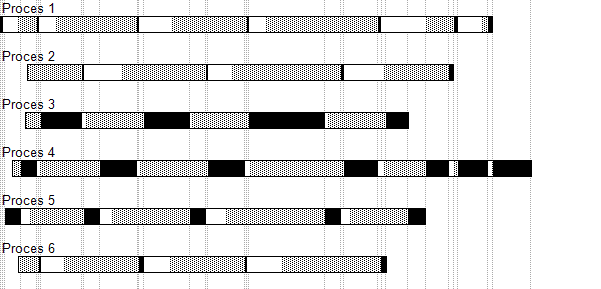
\includegraphics[width=\linewidth]{images/schedule_fcfs.png}
  \caption{First come first served}
  \label{fig:schedfcfs}
  \centering
  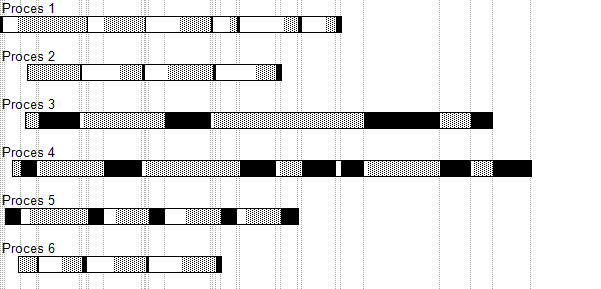
\includegraphics[width=\linewidth]{images/schedule_sjf.png}
  \caption{Shortest job first}
  \label{fig:schedsjf}
  \centering
  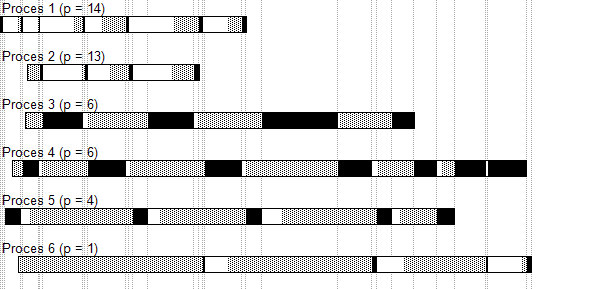
\includegraphics[width=\linewidth]{images/schedule_ps_noqua_age.png}
  \caption{Priority scheduling (niet-pre\"emptief, met aging)}
  \label{fig:schedpsnopre}
  
\includegraphics[width=0.8\linewidth]{images/legende.png}
\end{figure}

\section{Pre\"emptieve Scheduling-strategie\"en}

Naast de niet-pre\"emptieve strategie\"en die in de vorige sectie besproken werden, bestaan er natuurlijk ook pre\"emptieve algoritmes. Hier zal het besturingssysteem de controle van de processor kunnen terugeisen, ook al is het actieve programma nog niet klaar. In het schema van de toestanden van een proces, is er hier dus w\'el een overgang van `actief' naar `gereed'. In deze sectie bekijken we de pre\"emptieve versies van de drie scheduling-strategie\"en die we eerder besproken hebben.

\subsection{Hardware-ondersteuning}

Om een pre\"emptief algoritme te schrijven, is hardware-ondersteuning nodig. Eenmaal de scheduler een proces actief gemaakt heeft, krijgt dat proces de controle over de processor. Het besturingssysteem is op dat moment niet meer actief. Het proces kan in principe dus blijven rekenen (of vastzitten in een oneindige lus omwille van een programmeerfout), zonder dat er een oproep gedaan wordt naar het besturingssysteem. Op een of andere manier moet het besturingssysteem dus de mogelijkheid hebben om de controle over de processor terug te krijgen, zonder dat het proces meewerkt. Dit kan door gebruik te maken van de interrupt-functionaliteiten die al eerder beschreven werden in hoofdstuk~\ref{chap:basis}.

De lijst van \emph{soorten interrupts} (sectie~\ref{sec:soorten}) geeft aan dat er een klok interrupt is die de processor zelf genereert wanneer er een bepaalde tijdsperiode verstreken is. Een scheduling-algoritme kan dan deze klok instellen net voordat het een nieuw proces actief maakt. Wanneer het proces begint te rekenen en de controle van de processor behoudt, zal uiteindelijk de klok aflopen en de processor de bijhorende klok-interrupt genereren. Hierdoor wordt het interrupt-mechanisme opgeroepen en krijgt het besturingssysteem de kans om de interrupt af te handelen. In dit geval zal het besturingssysteem dan zien dat het quantum van het actieve proces afgelopen is, en dat een nieuw proces moet geactiveerd worden.

\subsection{Round Robin}

Het \emph{round robin}\index{round robin}-algoritme past dezelfde strategie toe als het FCFS-algoritme, maar dwingt voor elk proces een maximale uitvoertijd af. Een proces dat geselecteerd wordt om uit te voeren krijgt dus een bepaalde hoeveelheid tijd toegewezen waarin het de processor mag gebruiken. Het tijdsbestek waarin het proces actief mag zijn, wordt ook een \emph{time slice}\index{time slice} of een \emph{quantum}\index{quantum} genoemd.

Wanneer het proces blokkeert (bijv. omdat het een bestand wil lezen) voordat zijn quantum afgelopen is, zal het scheduling-algoritme het proces in de lijst van geblokkeerde processen steken. Het eerstvolgende proces dat gereed is wordt dan gekozen en actief gemaakt. Indien het proces blijft rekenen totdat zijn quantum afloopt, dan zal de scheduler het proces onderbreken en achteraan in de lijst steken van processen die gereed zijn. Het eerstvolgende proces dat gereerd is wordt dan uit de lijst gehaald en actief gemaakt. Merk op dat dit hetzelfde proces kan zijn, in het geval er verder geen processen gereed zijn.

Net als het FCFS-algoritme is round robin een eerlijk algoritme zonder starvation. Omwille van de korte quantums zal een proces de processor ook nooit voor lange tijd kunnen opeisen. Hierdoor zal elk proces snel aan de beurt komen, wat de responstijd van het algortime sterk verbetert. Langs de andere kant zorgt het frequente wisselen van processen weer voor een extra overhead en zal de doorvoer iets minder goed zijn dan bij FCFS. Figuur~\ref{fig:schedrr} toont de uitvoer van het round robin-algoritme\footnote{Merk op dat in de figuur het wisselen tussen processen geen vertraging oplevert. Hierdoor lijkt de throughput van round robin hetzelfde als bij FCFS, maar dit is natuurlijk niet realistisch.}. Vergelijk deze figuur met de uitvoer van FCFS (figuur~\ref{fig:schedfcfs}) en verifieer dat voor korte processen (bijv. proces 1) de responstijd veel korter is bij round robin dan bij FCFS.

Een belangrijke keuze die de ontwikkelaar van het besturingssysteem moet maken, is de keuze van de lengte van de tijdsquantums. Kortere tijdsquantums zorgen er voor dat de responstijd van de processen verbetert, maar zorgt ook voor meer overhead omdat er vaker moet gewisseld worden tussen processen. Hoe langer de quantums worden, hoe meer het algoritme op FCFS begint te lijken. Men kan zeggen dat FCFS eigenlijk round robin is waarbij de tijdsquantums oneindig lang zijn.

\subsection{Shortest Remaining Time}

Het shortest job first-algoritme uit sectie~\ref{sec:sjf} probeert de gemiddelde wachttijd en omlooptijd van de processen te minimaliseren door korte processen voorrang te geven op langere processen (t.t.z., het geeft processen voorrang waarvan het algoritme \emph{denkt} dat ze het kortst zullen uitvoeren). SJF is echter niet-pre\"emptief, wat betekent dat wanneer er een proces geselecteerd is dat het niet meer onderbroken wordt totdat het zelf de processor teruggeeft.

Stel dat er slechts \'e\'en proces klaar is en dat dit proces zeer lang moet uitvoeren. Het SJF-algoritme gaat natuurlijk dit proces activeren, omdat er geen enkel ander proces klaar is. Stel dat n\'et nadat het proces geactiveerd is, er een tweede (en veel korter) proces klaar is om uitgevoerd te worden. Dit korte proces zal moeten wachten totdat het langere proces uitgevoerd is, alhoewel het eigenlijk beter is dat het actieve proces onderbroken wordt en het korte proces voorrang krijgt.

Het shortest remaining time-algoritme is een pre\"emptieve versie van het SJF-algoritme. Wanneer een nieuw proces geactiveerd moet worden, zal SRT --- net zoals SJF --- het proces activeren waarvan verwacht wordt dat het het kortst gaat uitvoeren. Wanneer er echter een nieuw proces in de ready queue gezet wordt, zal SRT nagaan of het nieuwe proces korter is dan de verwachte resterende uitvoertijd van het actieve proces. Indien het nieuwe proces korter is, zal dat geactiveerd worden.

\begin{figure}
\centering
  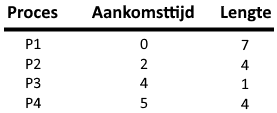
\includegraphics[width=0.5\linewidth]{images/srtsjfvgl-1.png}
  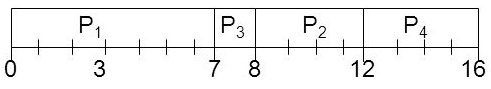
\includegraphics[width=0.75\linewidth]{images/srtsjfvgl-sjf.png}
  \caption{De uitvoering van de processen, volgens shortest job first}\label{fig:execsjf}
  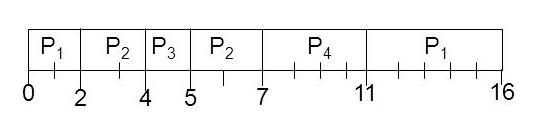
\includegraphics[width=0.75\linewidth]{images/srtsjfvgl-srt.png}
  \caption{De uitvoering van de processen, volgens shortest remaining time}\label{fig:execsrt}
\end{figure}

Figuren~\ref{fig:execsjf} en \ref{fig:execsrt} tonen het verschil in uitvoer tussen respectievelijk het SJF- en SRT-algoritme. De processen in figuur~\ref{fig:execsjf} worden niet meer onderbroken eenmaal ze geactiveerd zijn, wat op tijdstip 2 leidt tot een niet-optimale situatie. Wanneer proces 2 binnenkomt, moet proces 1 nog 5 tijdseenheden uitvoeren. Het SRT-algoritme in figuur~\ref{fig:execsrt} zal op dat punt de processor geven aan proces 2. Als we de gemiddelde wachttijd berekenen voor beide algoritmes, komen we uit op een gemiddelde wachttijd van 4 tijdseenheden voor SJF, tegen 3 tijdseenheden voor SRT (reken na!).

\subsection{Priority Scheduling}

Een nadeel van de niet-pre\"emptieve versie van het priority scheduling algoritme is dat een lang lage-prioriteitsproces de processor voor grote stukken tijd kan controleren. Processen met een hogere prioriteit zullen dan moeten wachten totdat het actieve lage-prioriteitsproces afgewerkt is. Dit probleem kan eenvoudig opgelost worden door hoge-prioriteitsprocessen voorrang te geven op processen met lagere prioriteit. Ook wanneer twee processen dezelfde prioriteit hebben, moet er afgewisseld worden. Figuur~\ref{fig:schedpspre} toont de werking van dit aangepast algoritme. Merk op dat we ook hier het probleem van starvation moeten oplossen door gebruik te maken van aging.

\begin{figure}
\centering
  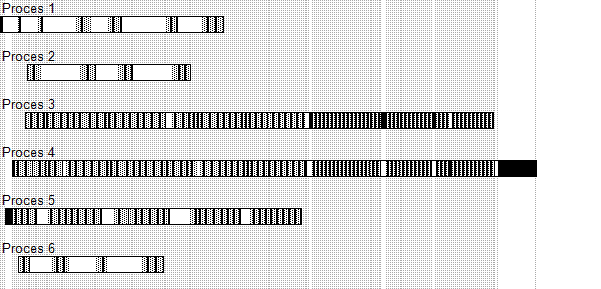
\includegraphics[width=\linewidth]{images/schedule_rr.png}
  \caption{Round robin}
  \label{fig:schedrr}
  \centering
  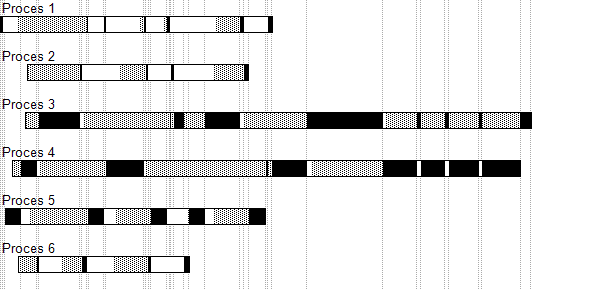
\includegraphics[width=\linewidth]{images/schedule_srt.png}
  \caption{Shortest remaining time}
  \label{fig:schedsrt}
  \centering
  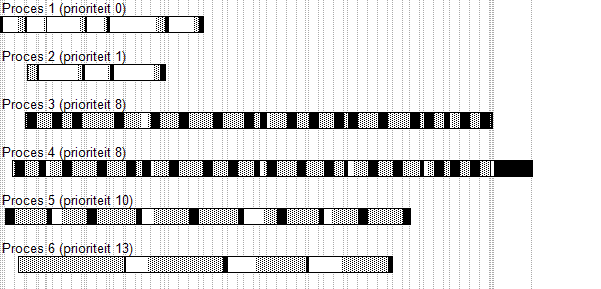
\includegraphics[width=\linewidth]{images/schedule_ps_qua_age.png}
  \caption{Priority scheduling (met aging)}
  \label{fig:schedpspre}
  
\includegraphics[width=0.8\linewidth]{images/legende.png}
\end{figure}


%\section{Voorbeeld: de Windows scheduler}
%\TODO{aanvullen}
%Numa cores
%Energiebeheer
%Variabele klokfrequentie
% https://msdn.microsoft.com/en-us/library/windows/desktop/ms685096(v=vs.85).aspx
% https://pdfs.semanticscholar.org/presentation/132c/457aad36535a4764ec1a2ee6f219c2e1df46.pdf
% http://www.i.u-tokyo.ac.jp/edu/training/ss/lecture/new-documents/Lectures/03-ThreadScheduling/ThreadScheduling.pdf 